RC, står for Resistor og Kapasitor (motstand og kondensator).
Og en RC-krets er simpelthen kretser
som består av motstander og kondensatorer.

\begin{circuitikz} \draw
(0,0) to[vsourcesin] (0,2)
      to[R] (4,2)
      to[C] (4,0)
      -- (0,0)
      ;
\end{circuitikz}



\paragraph{Spenning og impedans} \mbox{} \\
Husk at strømmen i en kondensator ligger 90 grader forran spenningen.
Det vil si at spenningen over en kondensator ligger forskøvet
90 grader i forhold til spenningen i en motstand.
Vektorsummen gir den totale spenningen.
\\
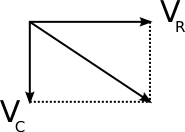
\includegraphics[width=0.25\textwidth]{./img/spenningRC}
\\
I en krets med en motstand og en kondensator i serie gir dette oss
$$V_T = \sqrt{V_R^2 + V_C^2}$$
Og tilsvarende for impedansen.
$$Z_T = \sqrt{R^2 + X_C^2}$$



\paragraph{Tidskonstant} \mbox{} \\
TODO
